\documentclass[10pt,english,aspectratio=169]{beamer}
% Use notes or hide notes or show only notes or handout


\usetheme{default}

\usepackage{xstring}
\usepackage{pgfpages}
%\makeatletter
%\IfSubStr{\@classoptionslist}{handout}
%  {\pgfpagesuselayout{2 on 1}[letterpaper,border shrink=5mm]}
%  {}
%\makeatother

\usepackage{amsmath,amssymb,amsthm}
\usepackage{stmaryrd}
\usepackage{enumerate}
\usepackage{stfloats}
\usepackage{bbm}
\usepackage{pdfpages}
\usepackage{framed}
\usepackage{tabularx}
\usepackage{scalerel}

\usepackage[most]{tcolorbox}
\tcbset{highlight math style={enhanced,
  colframe=white,colback=yellow!15,arc=8pt,boxrule=1pt,
  }}
  
\usepackage{tikz,pgf,pgfplots}
\usepackage{algorithm,algorithmic}
\usepgflibrary{shapes}
\usetikzlibrary{%
  arrows,%
  arrows.meta,
  backgrounds,
  shapes.misc,% wg. rounded rectangle
  shapes.arrows,%
  shapes,%
  calc,%
  chains,%
  matrix,%
  positioning,% wg. " of "
  scopes,%
  decorations.pathmorphing,% /pgf/decoration/random steps | erste Graphik
  shadows,%
  backgrounds,%
  fit,%
  petri,%
  quotes
}

\tikzset{background rectangle/.style={
    fill=white,
  },
  use background/.style={    
    show background rectangle
  }
}

\setbeamersize{text margin left=10mm,text margin right=35mm}

\pgfplotsset{compat=1.12}

%\usetheme{Frankfurt}
%\usecolortheme{ldpc}
\useinnertheme{rounded}
\usecolortheme{whale}
\usecolortheme{orchid}

\newcommand{\ul}[1]{\underline{#1}}
\renewcommand{\Pr}{\mathbb{P}}

%% Setup slides and notes
\makeatletter
\IfSubStr{\@classoptionslist}{notes} { \IfSubStr{\@classoptionslist}{hide} {}{\IfSubStr{\@classoptionslist}{only} {}{\setbeameroption{show notes on second screen=right}}} }{}
\makeatother
%\setbeamertemplate{note page}{\pagecolor{yellow!5}\vfill\insertnote\vfill}

\newcommand{\getpdfpages}[2]{\begingroup
  \setbeamercolor{background canvas}{bg=}
  \addtocounter{framenumber}{1}
  \includepdf[pages={#1},%
  pagecommand={%
    \expandafter\def\expandafter\insertshorttitle\expandafter{%
      \insertshorttitle\hfill\insertframenumber\,/\,\inserttotalframenumber}}%
  ]{#2}
  \endgroup}

\newcommand{\backupbegin}{
   \newcounter{finalframe}
   \setcounter{finalframe}{\value{framenumber}}
}
\newcommand{\backupend}{
   \setcounter{framenumber}{\value{finalframe}}
}

 \setbeamercolor{bibliography entry author}{fg=black}
 \setbeamercolor{bibliography entry title}{fg=black}
 \setbeamercolor{bibliography entry location}{fg=black}
 \setbeamercolor{bibliography entry note}{fg=black}
 
 \setbeamerfont{bibliography item}{size=\footnotesize}
 \setbeamerfont{bibliography entry author}{size=\footnotesize}
 \setbeamerfont{bibliography entry title}{size=\footnotesize}
 \setbeamerfont{bibliography entry location}{size=\footnotesize}
 \setbeamerfont{bibliography entry note}{size=\footnotesize}
 \setbeamertemplate{bibliography item}{\insertbiblabel}
 
\newlength\tikzwidth
\newlength\tikzheight


\newcommand{\mc}[1]{\mathcal{#1}}
\newcommand{\mbb}[1]{\mathbb{#1}}
%\newcommand{\expt}{\mbb{E}}
%\newcommand{\dd}{\mathrm{d}}
\newcommand{\Interior}[1]{\ensuremath{{#1}^{\circ}}}
\newcommand{\Closure}[1]{\ensuremath{\overline{#1}}}
\newcommand{\Complement}[1]{\ensuremath{{#1}^{c}}}

\newcommand{\Expect}{\ensuremath{\mathrm{E}}}
\newcommand{\vecnot}{\underline}
\newcommand{\RealNumbers}{\ensuremath{\mathbb{R}}}
\newcommand{\RationalNumbers}{\mathbb{Q}}
\newcommand{\ComplexNumbers}{\mathbb{C}}
\newcommand{\Real}{\mathrm{Re}}
\newcommand{\Span}{\mathrm{span}}
\newcommand{\Rank}{\mathrm{rank}}
\newcommand{\Nullity}{\mathrm{nullity}}
\newcommand{\Trace}{\mathrm{tr}}
\newcommand{\Diag}{\mathrm{diag}}
\newcommand{\dd}{\mathrm{d}}
\DeclareMathOperator*{\esssup}{ess\,sup}

% Use < , > inner product
\newcommand{\inner}[2]{{\left\langle #1 \mskip2mu , #2 \right\rangle}}
\newcommand{\tinner}[2]{{\langle #1 \mskip1mu , #2 \rangle}}

% Use < | > inner product
%\newcommand{\inner}[2]{{\left\langle #1 \mskip2mu \middle| \mskip2mu #2 \right\rangle}}
%\newcommand{\tinner}[2]{{\langle #1 \mskip1mu | \mskip1mu  #2 \rangle}}




\def\checkmark{\tikz\fill[scale=0.4](0,.35) -- (.25,0) -- (1,.7) -- (.25,.15) -- cycle;}
\def\greencheck{{\color{green}\checkmark}}
\def\scalecheck{\resizebox{\widthof{\checkmark}*\ratio{\widthof{x}}{\widthof{\normalsize x}}}{!}{\checkmark}}
\def\xmark{\tikz [x=1.4ex,y=1.4ex,line width=.2ex, red] \draw (0,0) -- (1,1) (0,1) -- (1,0);}
\def\redx{{\color{red}\xmark}}

\renewcommand{\footnotesep}{-2pt}


\begin{document}

\title{ECE 586: Vector Space Methods \\ Lecture 21: Projection onto Convex Sets}
\author{Henry D. Pfister \\ Duke University}
\date{}
%\date{August 20th, 2020}
%\maketitle

\setbeamertemplate{navigation symbols}{}

\begin{frame}[plain]
	\titlepage
	
	\note{
		\vspace{8mm}
		\begin{enumerate}
			\setlength\itemsep{3mm}
			\color{red}
			\item Welcome to the 11th video lecture for ECE 586, Vector Space Methods. \\[2mm]
			Today, we'll finish our discussion of subspaces and bases and then move on to linear transforms.
		\end{enumerate}
	}
\end{frame}

\addtocounter{framenumber}{-1}
\setbeamertemplate{navigation symbols}{\textcolor{blue}{\footnotesize \insertframenumber ~/ \inserttotalframenumber}}






\begin{frame}{5.3: Convexity}

\vspace{-1mm}

\begin{minipage}{0.75\textwidth}
Convexity is a useful property defined for sets, spaces, and functionals that simplifies analysis and optimization.

\begin{definition}[convex set]
Let $V$ be a vector space over $\RealNumbers$.
The subset $A \subseteq V$ is called a \textcolor{blue}{convex set} if, for all $\vecnot{a}_1,\vecnot{a}_2 \in A$ and $\lambda\in(0,1)$, we have $\lambda \vecnot{a}_1 + (1-\lambda) \vecnot{a}_2 \in A$.
It is \textcolor{blue}{strictly convex} if, for all $\vecnot{a}_1,\vecnot{a}_2 \in \Closure{A}$ and $\lambda\in(0,1)$,
%we have
$\lambda \vecnot{a}_1 + (1-\lambda) \vecnot{a}_2 \in \Interior{A}$.
\end{definition}
\end{minipage}
\hfill
\begin{minipage}{0.22\textwidth}
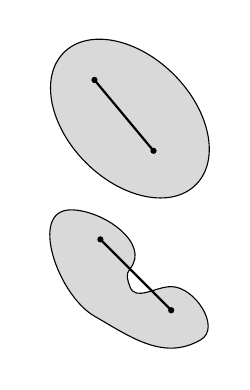
\begin{tikzpicture}[rotate=270,scale=0.75]
    \draw[rotate=-45,fill=gray!30] (-1.8,-1.8) ellipse (30pt and 45pt);
    \draw[thick] (-3.2,-0.6) -- (-2.0,0.4);
    \fill (-3.2,-0.6) circle[radius=1.5pt];
    \fill (-2.0,0.4) circle[radius=1.5pt];
    
    \draw[fill=gray!30] (0,0) to [out=140,in=90] (-1,-1)
    to [out=-90,in=240] (0.8,-0.6)
    to [out=60,in=-60] (1.2,1.2)
    to [out=120,in=90] (0.3,0.7)
    to [out=-90,in=20] (0.3,0)
    to [out=200,in=-40] (0,0);
    \draw[thick] (-0.5,-0.5) -- (0.7,0.7);
    \fill (-0.5,-0.5) circle[radius=1.5pt];
    \fill (0.7,0.7) circle[radius=1.5pt];
\end{tikzpicture}
\end{minipage}

\begin{definition}[convex function]<2->
\begin{minipage}{0.70\textwidth}
Let $V$ be a vector space, $A \subseteq V$ be a convex set, and $f \colon V \rightarrow \RealNumbers$ be a functional.
The functional $f$ is called \textcolor{blue}{convex} on $A$ if, for all $\vecnot{a}_1,\vecnot{a}_2 \in A$ and $\lambda\in(0,1)$, \vspace{-1mm}
\[ f( \lambda \vecnot{a}_1 + (1-\lambda) \vecnot{a}_2 ) \leq \lambda f( \vecnot{a}_1 ) + (1-\lambda) f ( \vecnot{a}_2 ). \vspace{-1mm} \]
It is \textcolor{blue}{strictly convex} if equality implies $\vecnot{a}_1 = \vecnot{a}_2$.
\end{minipage}\hspace{-3mm}
\begin{minipage}{0.29\textwidth}
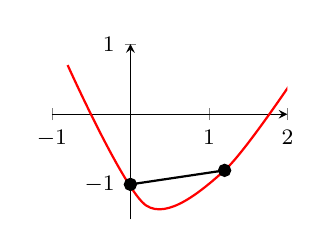
\begin{tikzpicture}
  \begin{axis}[axis x line=center,
    axis y line=center, small,width=1.8in,height=1.5in,xmin=-1,xmax=2,ymin=-1.5,ymax=1]
     \addplot[mark=*, thick, black] coordinates {(0,-1)(1.2,-0.8)};
     \addplot[red,smooth,thick,-] coordinates  {
    (-0.8,0.7) (0.2,-1.3) (1.2,-0.8) (2.2,0.7)};
  \end{axis}
\end{tikzpicture}
\end{minipage}
\end{definition}

\end{frame}

\begin{frame}{5.3: Convex Optimization}

\begin{definition}
Let $(X,\|\cdot\|)$ be a normed vector space.
Then, a real functional $f \colon X \rightarrow \RealNumbers$ achieves a \textcolor{blue}{local minimum value} at $\vecnot{x}_0 \in X$ if: \\ \hspace{3mm}  there is an $\epsilon > 0$ such that, for all $\vecnot{x}\in X$ satisfying $\| \vecnot{x} - \vecnot{x}_0 \| < \epsilon$, we have  $f(\vecnot{x}) \geq f(\vecnot{x}_0)$.
If this lower bound holds for all $x\in X$, then the local minimum is also a \textcolor{blue}{global minimum value}.
\end{definition}

\vspace{2mm}

\begin{theorem}<2->
Let $(X,\|\cdot\|)$ be a normed vector space, $A \subseteq X$ be a convex set, and $f \colon X \rightarrow \RealNumbers$ be a convex functional on $A$.
Then, \textcolor{blue}{any local minimum value of $f$ on $A$ is a global minimum value on $A$}.
If the functional is strictly convex on $A$ and achieves a local minimum value on $A$, then there is a unique point $\vecnot{x}_0 \in A$ that achieves the global minimum value on $A$.
\end{theorem}

\vspace{1mm}

\visible<2->{Prove in live session and discuss strict convexity of induced norm squared}

\end{frame}

\begin{frame}{5.3: Convex Optimization and Derivatives}

\begin{minipage}{0.55\textwidth}
Let $(X,\|\cdot\|)$ be a normed vector space and $f \colon X \rightarrow \RealNumbers$ be a convex functional on a convex set $A \subseteq X$.
\end{minipage}
\begin{minipage}{0.44\textwidth}\hspace{3mm}
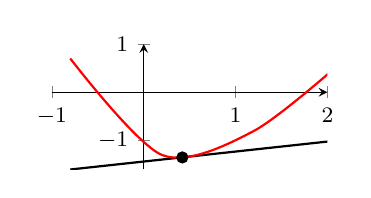
\begin{tikzpicture}
  \begin{axis}[axis x line=center,
    axis y line=center, small,width=2in,height=1.25in,xmin=-1,xmax=2,ymin=-1.6,ymax=1]
     \addplot[mark=none, thick, black] coordinates {(-0.8,-1.6)(2.2,-0.98)};
     \addplot[red,smooth,thick,-] coordinates  {
    (-0.8,0.7) (0.2,-1.3) (1.2,-0.8) (2.2,0.7)};
    \addplot[mark=*] coordinates {(0.42,-1.35)};
  \end{axis}
\end{tikzpicture}
\end{minipage}

\begin{theorem}
If $f$ has a directional derivative  at $\vecnot{x}_0 \in A$ in the direction $\vecnot{x}-\vecnot{x}_0$, then \vspace{-1mm}
\[ f(\vecnot{x}) \geq f(\vecnot{x}_0) + \delta f (\vecnot{x}_0;\vecnot{x}-\vecnot{x}_0) %f'(\vecnot{x}_0)(\vecnot{x}-\vecnot{x}_0) 
\vspace{-1mm} \]
for all $\vecnot{x}\in A$.
If $f$ is strictly convex then the inequality is strict for $\vecnot{x}\neq \vecnot{x}_0$.
\end{theorem}

\vspace{1mm}

\begin{corollary}<2->
If $f$ has directional derivatives in all directions at $\vecnot{x}_0 \in A$ and they all equal zero, then \vspace{-2mm}
\[ f(\vecnot{x}_0) = \min_{\vecnot{x}\in A} f(\vecnot{x}). \vspace{-2mm} \]
If $f$ is strictly convex, then $\vecnot{x}_0$ is the unique minimizer over $A$.
\end{corollary}

\visible<2->{Prove corollary in live session}

\end{frame}


\begin{frame}{4.6: Projection onto Convex Sets}

\begin{minipage}{0.44\textwidth}
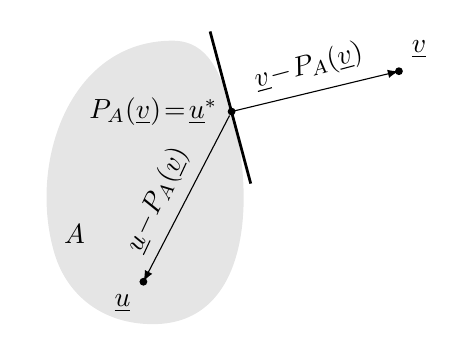
\begin{tikzpicture}[yscale=0.9,bullet/.style={circle,fill,inner sep=1.00pt,node contents={}}]
 \draw[-latex] (0,0) node[bullet,label=left:{$P_A(\vecnot{v}) \!=\! \vecnot{u}^*$},alias=PC]  -- (15:2.2) node[midway,sloped,above=0.25mm] {$\vecnot{v}\!-\! P_A(\vecnot{v})$}
    node[bullet,label=above right:$\vecnot{v}$,alias=v];
\draw[-latex] (PC) -- ++ (-115:2.65) node[pos=0.57,above=0.25mm,sloped]{$\vecnot{u}\!-\! P_A(\vecnot{v})$}     node[bullet,label=below left:$\vecnot{u}$];
\fill[black,fill,opacity=0.1] (PC) to[out=105,in=0] ++ (-0.75,1) to[out=180,in=105] ++ (-1.5,-3)
 node[above right,opacity=1]{$A$} to[out=-75,in=180] ++ (1.25,-1) to[out=0,in=-75] node[sloped, inner xsep=10mm, inner ysep=0, opacity=1, fill=black, pos=0.999] {} cycle;
\end{tikzpicture}
\end{minipage}
\begin{minipage}{0.55\textwidth}
\hspace{3mm} The projection of vectors onto subspaces can be generalized to convex sets\\[-2mm]

For Hilbert space $V$ and closed convex set $A\subseteq V$, let $P_{A}:V\rightarrow A$ denote the orthogonal projection of $\vecnot{v}\in V$ onto $A$: \vspace{-1mm}
\[
P_A (\vecnot{v}) \triangleq \arg \min_{\vecnot u\in A}\left\Vert \vecnot u-\vecnot v\right\Vert \vspace{-1mm} 
\]
\end{minipage}

\begin{theorem}<1->
The orthogonal projection of $\vecnot v\in V$ onto a closed convex set $A\subseteq V$ exists and is unique.
\end{theorem}

\begin{theorem}<2->
For any $\vecnot{v} \notin A$, we have $\vecnot{u}^* = P_A (\vecnot{v})$ iff $\tinner{ \vecnot{v}-\vecnot{u}^* \,}{\, \vecnot{u}-\vecnot{u}^* } \leq 0$ for all $\vecnot{u}\in A$.
\end{theorem}

\visible<3->{Prove theorem in live session for compact $A$ via convex optimization}
\end{frame}

\begin{frame} \frametitle{Next Steps}

\begin{itemize}
\setlength\itemsep{5mm}
\item To continue studying after this video -- \vspace{2mm}

\begin{itemize}
 \setlength\itemsep{3mm}
 
 \item Try the required reading:  Course Notes EF 4.6, 5.2 - 5.3

 \item Also, look at the problems in Assignments 8 and 9
\end{itemize}
\end{itemize}

\note{
	\vspace{8mm}
	\begin{enumerate}
		\setlength\itemsep{3mm}
		\color{red}
		\item Here are some options to continue learning this material. (read) \\ [2mm]  That's it for today.  So, I'll see you next time.
	\end{enumerate}
}

\end{frame}

\end{document}


